\section{Discussion and Limitations}
\label{sec:discussion}
\label{sec:limitations}

Our measurements inform two memory-manager decisions without implementing
either: what to keep after an episode and what to show at each later step.
\emph{Retention} would require combining task-conditioned utility profiles with
an anticipated future-task distribution and memory costs; our measurements
characterize a defined evaluation task set, not a deployed agent's future
return. \emph{Exposure} is the standard retrieval problem: generic retrieval
recovers screen-defined answer-bearing memories far above chance but usually
not in its top ten (Section~\ref{sec:similarity}), so a reliable locator remains
open. For representation, the evaluated compressed representations retain less
answer-bearing text and gain less than Raw, including when total context is
fixed.

\paragraph{The pairing is constructed.}
The memories are real trajectory spans, but their pairing to tasks is a seeded
rule fixed before measurement, so every rate describes a defined evaluation task set rather than naturally
occurring future tasks. The observed harm rates should therefore not be
interpreted as population rates for deployed memory systems.

\begin{figure}[t]
\centering
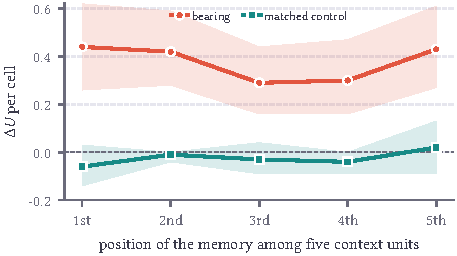
\includegraphics[width=\columnwidth]{fig_position}
\caption{Position affects per-pair measurements; the aggregate bearing--control
contrast remains positive after position standardization (exploratory). Per-cell $\Delta U$ by the memory's position among the five
context units in the second-session run, with task-clustered 95\% bands: the
bearing effect dips in the middle and recovers at the end, while the control
stays near zero at every position.}
\label{fig:position}
\Description{A line chart over five positions. The bearing line is about 0.44 and 0.42 at the first two positions, about 0.29 and 0.30 in the middle, and 0.43 at the last, with a wide band; the control line stays near zero throughout.}
\end{figure}

\paragraph{Session and position variance.}
Re-issuing $\lfDriftN$ byte-identical no-memory requests a day later changed
$\lfDriftReward$ rewards, so we compare only arms executed in one session. We then
measured both sources, session and position, directly by re-running the headline cells in a new session
with position redrawn per replicate (Section~\ref{sec:screened}). The aggregate
contrast keeps its direction. Single cells move (Figure~\ref{fig:cells}a). Position alone changes
$\soPosChgPct\%$ of labels and accounts for $\soPosVarPct\%$ of the variance of
$\Delta U$, and the bearing effect is weaker in the middle of the context
($\soPosMid$) than at its ends ($\soPosEdge$; Figure~\ref{fig:position}),
echoing~\cite{lostmiddle}. Labels agree with the original run at
$\kappa = \soStabSameK$ at the same position and $\soStabDiffK$ at a new one, and
changes almost always move to or from \emph{unchanged} (Figure~\ref{fig:cells}a). Standardizing the published contrast over position leaves it at
$\lfScrPosStd$.

\paragraph{Scope.}
The main results concern a single-call factual-recall reader evaluated on
the web and enterprise domains of LongMemEval-V2. The experiments use one
serving cluster and two reader checkpoints, limiting generalization to
other model families and deployments. The software-engineering and
scientific-coding evaluations show no measurable memory effect; the
positive factual-recall finding should not be extended to those settings. Single-item insertion cannot see
redundancy or complementarity between units, which Shapley-style attribution
could~\cite{meclear}. Our filler
comes from trajectories that host no bearing memory, so it never contains
competing evidence; realistic retrieval would, which likely makes our bearing
effect larger than a deployed system would see. Our leakage-audit rates are lower bounds (\supp{sec:extlimits}).

\paragraph{Release and reproducibility.}
\label{sec:release}
The Conditional Memory Utility Dataset is publicly available on
\href{https://huggingface.co/datasets/AgentsSci/AAMAS2027-ConditionalMemory}{Hugging Face}.
The frozen \texttt{v0.6-}\allowbreak\texttt{length-control} snapshot contains 16,816 evaluation
records, with paired outcomes, costs and available text, plus schema and
validation code. The data card documents the included conditions, missing
records and text withheld under upstream restrictions. This versioned snapshot
does not cover every later manuscript analysis, including the fixed-total-context
experiment. Per-pair labels depend on the evaluation condition; they are
observations, not unconditional targets for training a memory gate.
See \supp{sec:repro} for coverage and reuse details.

\paragraph{Conclusion.}
Evaluate memory compression by the task utility it preserves alongside its
costs. On LongMemEval-V2 factual-recall tasks, answer-bearing pairs gain more
than matched controls, and the tested summaries and structured records gain
less than Raw even at fixed total context, consistent with reduced retention
of relevant content. Our paired protocol makes these effects measurable
without exposing the future task to the memory writer. The headline contrast
stays positive across the tested sessions, positions and readers, while
individual labels remain condition-dependent. These factual-recall gains do
not extend to the tested coding benchmarks.
